\chapter{跨網路連線}
\section{設定連線步驟}
\begin{figure}[hbt!]
  \begin{center}
    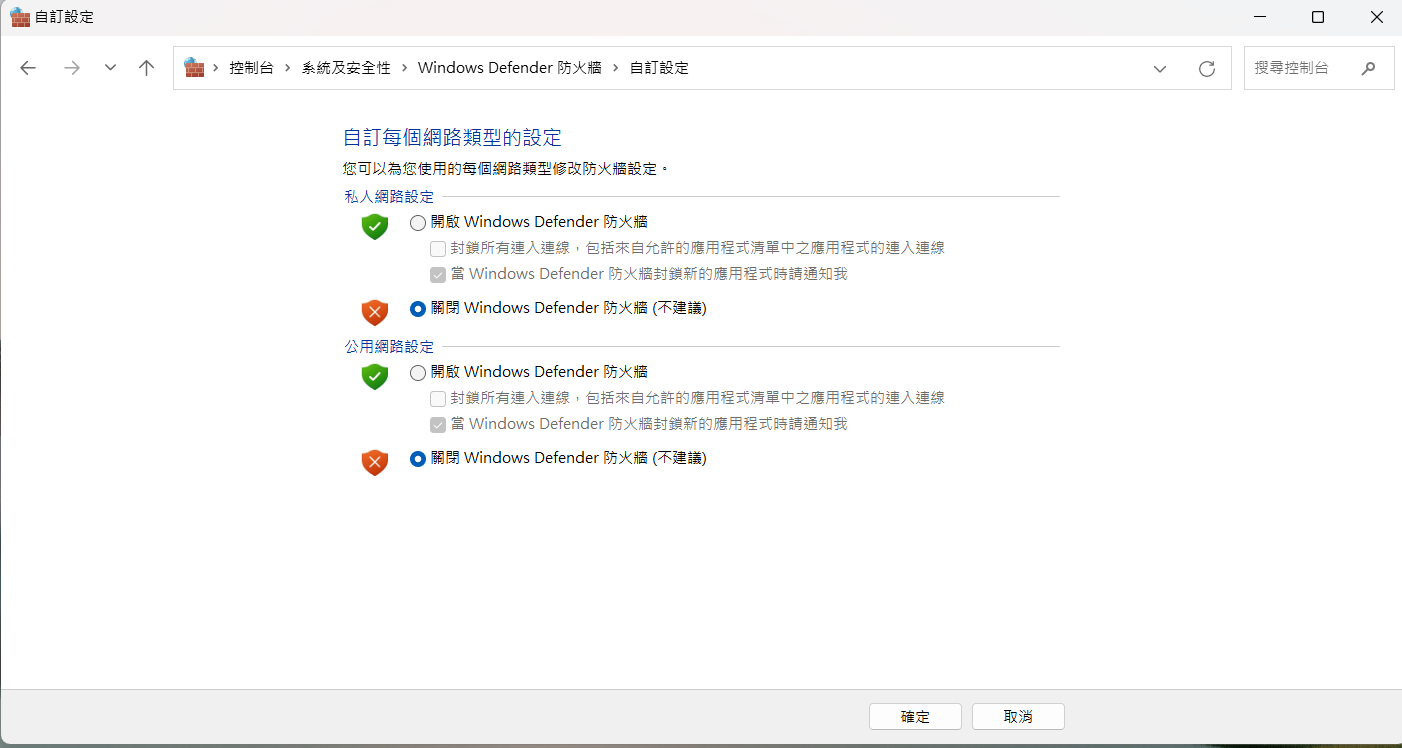
\includegraphics[width=0.5\textwidth]{連線_1.png}
  \end{center}
  \caption[關閉防火牆]{\phantomsection}
  \label{fig:photo}
\end{figure}

\begin{figure}[hbt!]
  \begin{center}
    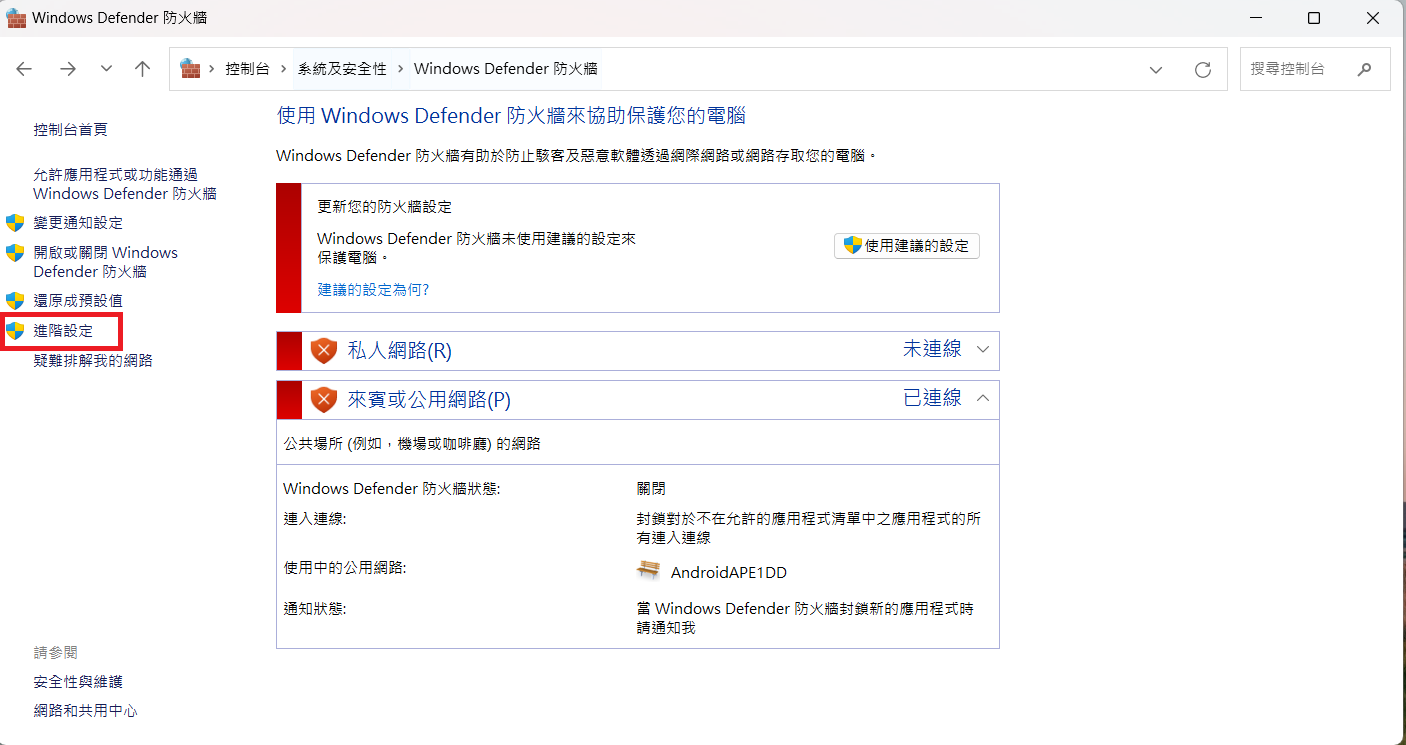
\includegraphics[width=0.5\textwidth]{連線_2.png}
  \end{center}
  \caption[點選進階設定]{\phantomsection}
  \label{fig:photo}
\end{figure}

\begin{figure}[hbt!]
  \begin{center}
    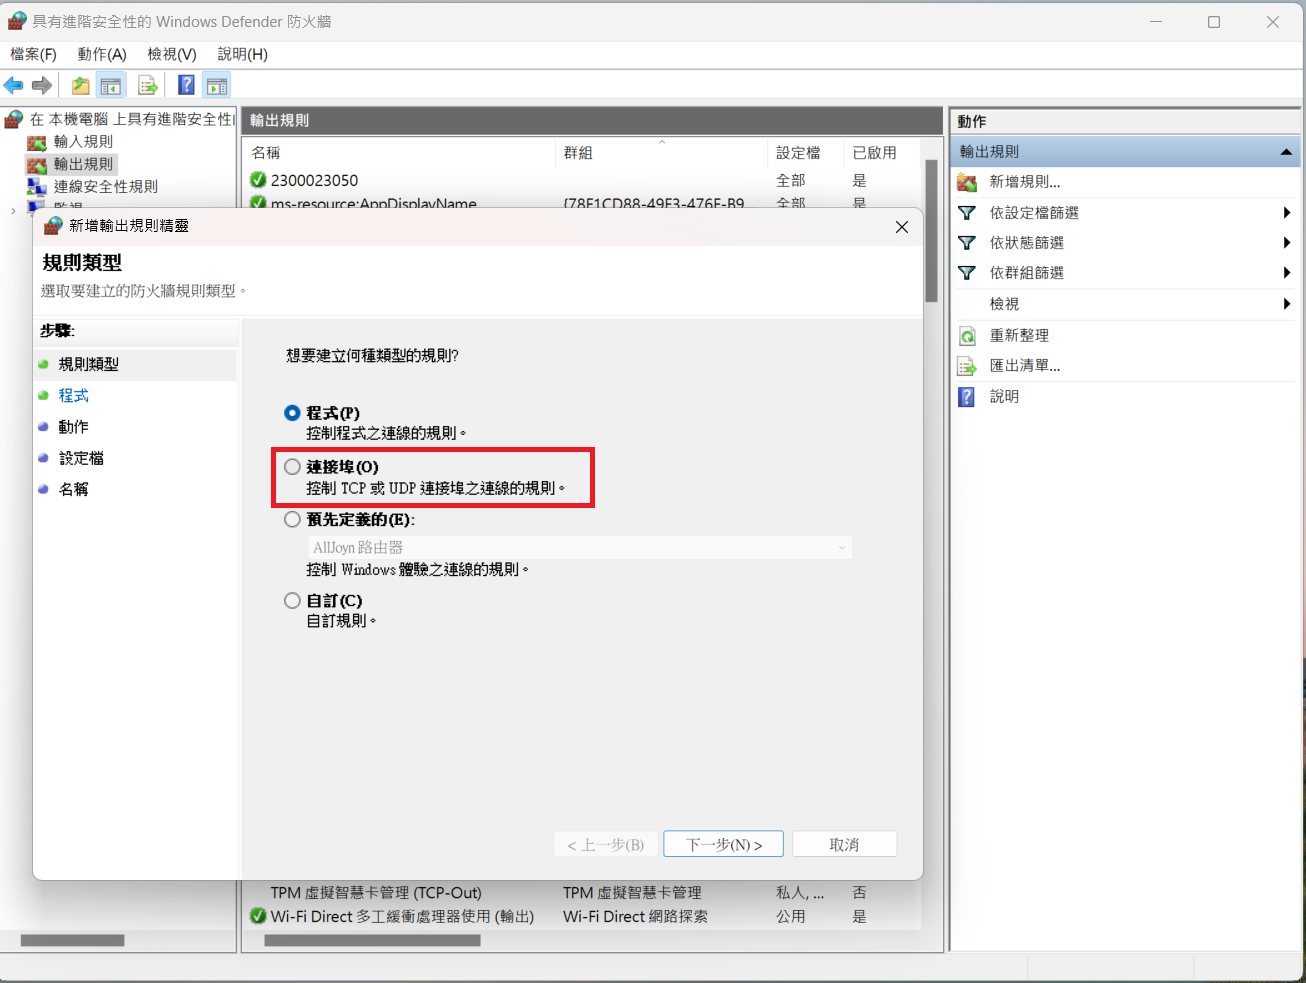
\includegraphics[width=0.5\textwidth]{連線_3.png}
  \end{center}
  \caption[設定輸入及輸出規則類型]{\phantomsection}
  \label{fig:photo}
\end{figure}

\begin{figure}[hbt!]
  \begin{center}
    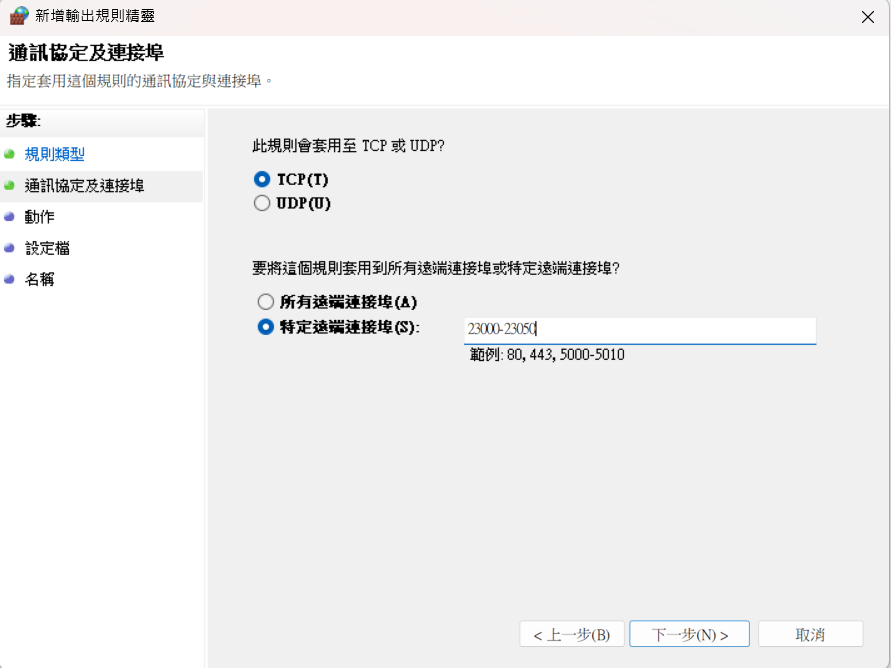
\includegraphics[width=0.5\textwidth]{連線_4.png}
  \end{center}
  \caption[設定特定遠端連接埠]{\phantomsection}
  \label{fig:photo}
\end{figure}

\begin{figure}[hbt!]
  \begin{center}
    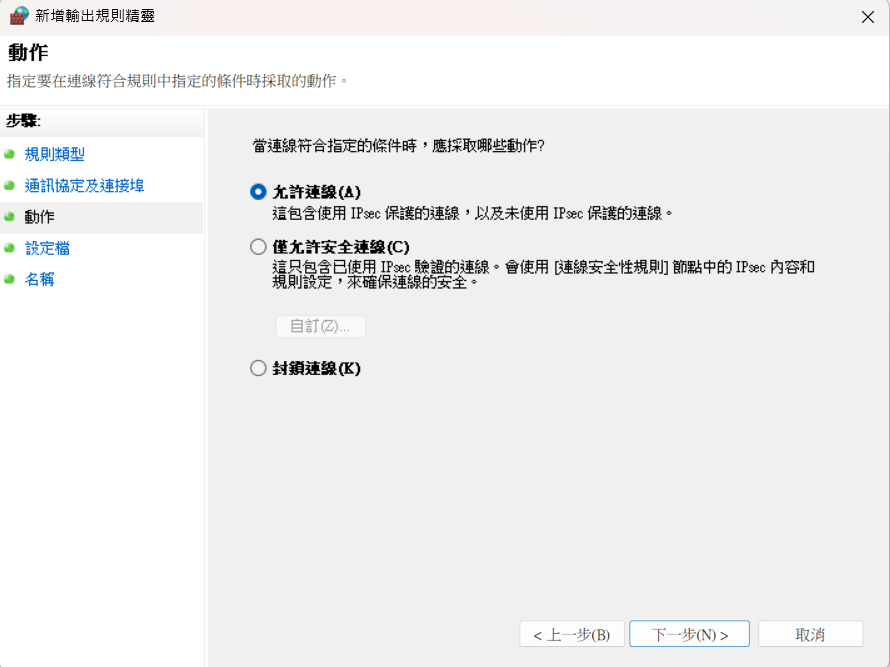
\includegraphics[width=0.5\textwidth]{連線_5.png}
  \end{center}
  \caption[v允許連線]{\phantomsection}
  \label{fig:photo}
\end{figure}

\begin{figure}[hbt!]
  \begin{center}
    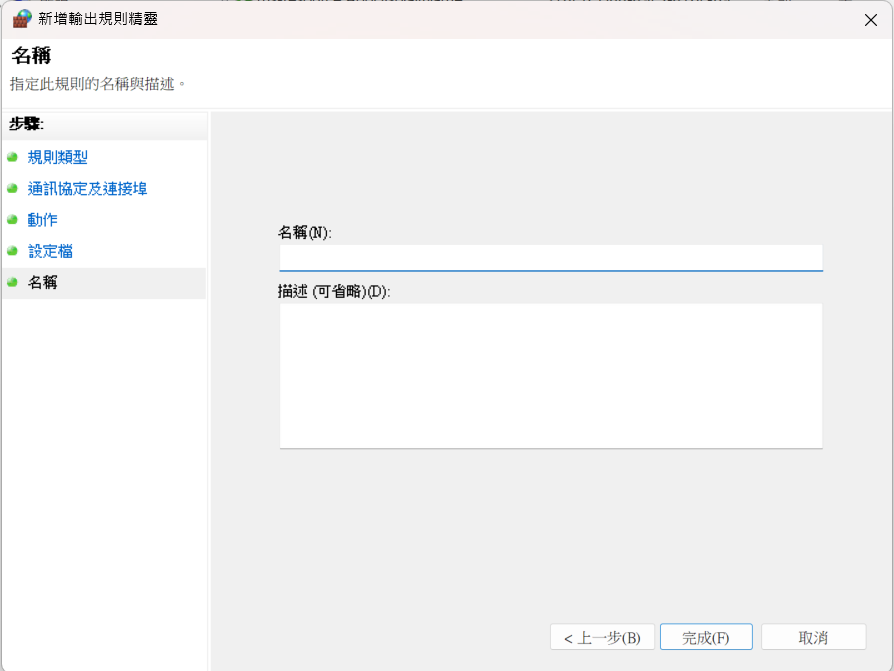
\includegraphics[width=0.5\textwidth]{連線_6.png}
  \end{center}
  \caption[設定名稱]{\phantomsection}
  \label{fig:photo}
\end{figure}

\begin{figure}[hbt!]
  \begin{center}
    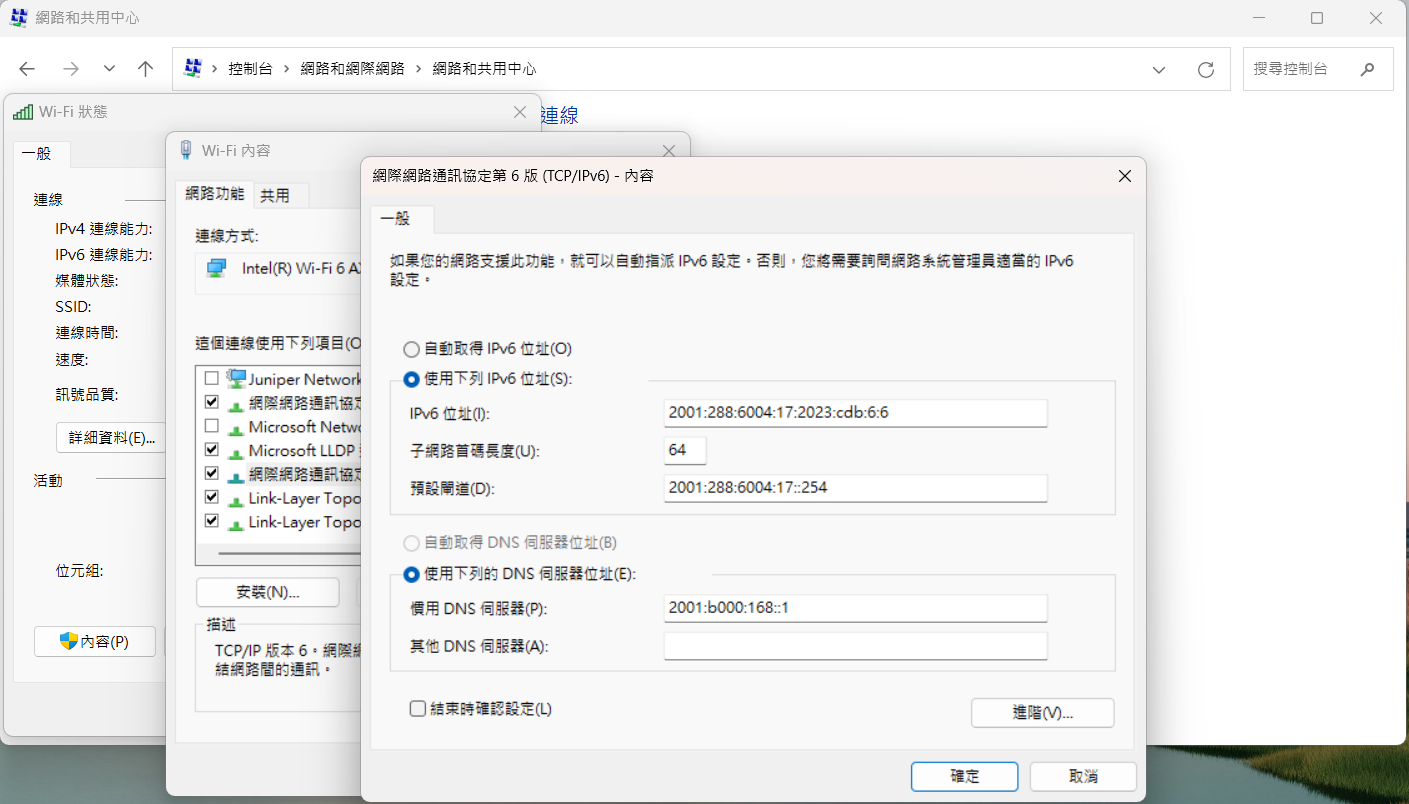
\includegraphics[width=0.5\textwidth]{連線_7.png}
  \end{center}
  \caption[設定規定的ipv6]{\phantomsection}
  \label{fig:photo}
\end{figure}

\newpage

\section{程式碼}
\begin{lstlisting}[language=Python, frame=single, numbers=left, captionpos=b, basicstyle=\ttfamily\small,showstringspaces=false, breaklines=true, tabsize=4, xleftmargin=15pt]
# pip install pyzmq cbor keyboard
from zmqRemoteApi import RemoteAPIClient
import keyboard

client = RemoteAPIClient('localhost', 23000)

print('Program started')
sim = client.getObject('sim')

sim.startSimulation()
print('Simulation started')

def setBubbleRobVelocity(leftWheelVelocity, rightWheelVelocity):
    leftMotor = sim.getObject('/leftMotor')
    rightMotor = sim.getObject('/rightMotor')
    sim.setJointTargetVelocity(leftMotor, leftWheelVelocity)
    sim.setJointTargetVelocity(rightMotor, rightWheelVelocity)

'''
# Example usage 1:
setBubbleRobVelocity(1.0, 1.0)
time.sleep(2)
setBubbleRobVelocity(0.0, 0.0)
'''
# use keyborad to move BubbleRob

while True:
    if keyboard.is_pressed('w'):
        setBubbleRobVelocity(1.0, 1.0)
    elif keyboard.is_pressed('s'):
        setBubbleRobVelocity(-1.0, -1.0)
    elif keyboard.is_pressed('a'):
        setBubbleRobVelocity(-1.0, 1.0)
    elif keyboard.is_pressed('d'):
        setBubbleRobVelocity(1.0, -1.0)
    elif keyboard.is_pressed('q'):
        # stop simulation
        sim.stopSimulation()
    else:
        setBubbleRobVelocity(0.0, 0.0)
\end{lstlisting}
